% % % % % % % % % % %
%-----------------------------------------------------------------------------
%
%               Template for sigplanconf LaTeX Class
%
% Name:         sigplanconf-template.tex
%
% Purpose:      A template for sigplanconf.cls, which is a LaTeX 2e class
%               file for SIGPLAN conference proceedings.
%
% Guide:        Refer to "Author's Guide to the ACM SIGPLAN Class,"
%               sigplanconf-guide.pdf
%
% Author:       Paul C. Anagnostopoulos
%               Windfall Software
%               978 371-2316
%               paul@windfall.com
%
% Created:      15 February 2005
%
%-----------------------------------------------------------------------------
\documentclass[preprint]{sigplanconf}

\usepackage{amsmath}

%\usepackage{biblatex}
%\usepackage[style=ieee]{biblatex}
%\AtEveryBibitem{%
%  \clearfield{issn} % Remove issn
%  \clearfield{doi} % Remove doi
%
%  \ifentrytype{online}{}{% Remove url except for @online
%    \clearfield{url}
%  }
%}

%\usepackage{pifont}
%\usepackage[T1]{fontenc} % this is just to get the natural encoding for the < > characters in text

\usepackage{color,soul}
\definecolor{highlight}{rgb}{1,1,0.6}
\definecolor{link}{rgb}{0.5,0.0,0.0}
\definecolor{cite}{rgb}{0.0,0.0,0.6}
\definecolor{url} {rgb}{0.3,0.0,0.3}
%\definecolor{grey}{rgb}{0.3,0.3,0.3}

\usepackage{algorithm}
\usepackage{algpseudocode}
\usepackage{listings}

\usepackage[hidelinks]{hyperref}
\hypersetup{
    colorlinks,
    linkcolor={cite},
    citecolor={cite},
    urlcolor ={cite}
}
\usepackage{enumitem}
\usepackage[british]{datetime2}

\usepackage{tabularx}
%\usepackage{array}
\usepackage{multirow}
\usepackage{booktabs}
%\newcolumntype{L}{>{\raggedright\arraybackslash}p{3cm}}
%\usepackage{dcolumn}
%\usepackage{multicol}

% % annotations environments % % 
\newcommand{\note}[1]{\textit{\textcolor{red}{\{#1\}}}}
\sethlcolor{highlight}


\def\ojoin{\setbox0=\hbox{$\bowtie$}%
  \rule[-.02ex]{.25em}{.4pt}\llap{\rule[\ht0]{.25em}{.4pt}}}
\def\leftouterjoin{\mathbin{\ojoin\mkern-5.8mu\bowtie}}
\def\rightouterjoin{\mathbin{\bowtie\mkern-5.8mu\ojoin}}
\def\fullouterjoin{\mathbin{\ojoin\mkern-5.8mu\bowtie\mkern-5.8mu\ojoin}}


%% PM Define authornote command for comments
\newcommand{\authornote}[1] {
    \begin{center}
        \framebox{
            {\begin{minipage}[t]{0.9\linewidth}
                \raggedright  \textbf{[PM]}~ \scriptsize #1 \normalsize
            \end{minipage}}
    }
    \end{center}
}

\usepackage{amssymb}
\let\oldemptyset\emptyset
\let\emptyset\varnothing

\usepackage{bm}
\usepackage{mathtools}
\def\filtcap{\mathrel{%
    \mathchoice{\FILTCAP}{\FILTCAP}{\scriptsize\FILTCAP}{\tiny\FILTCAP}%
}}
\def\FILTCAP{{%
    \setbox0\hbox{$\cap$}%
    \rlap{\hbox to \wd0{\hss$\circ$\hss}}\box0
}}


\newcommand{\structurenote}[2] {
    \begin{center}
        \framebox{
            \colorbox{purple!40}{\begin{minipage}[t]{0.9\linewidth}
                \raggedright  \textbf{[#1]}~ \scriptsize #2 \normalsize
            \end{minipage}}
    }
    \end{center}
}


%\usepackage{datetime}
%\usepackage[mark]{gitinfo2}

\newcommand{\prov}{\mathit{prov}}
\newcommand{\provs}{\texttt{PROV-S}}
\newcommand{\entity}{\texttt{entity}}
\newcommand{\cL}{{\cal L}}
\newcommand{\os}{\mathit{os}}
\newcommand{\is}{\mathit{i}s}



% The following \documentclass options may be useful:

% preprint       Remove this option only once the paper is in final form.
%  9pt           Set paper in  9-point type (instead of default 10-point)
% 11pt           Set paper in 11-point type (instead of default 10-point).
% numbers        Produce numeric citations with natbib (instead of default author/year).
% authorversion  Prepare an author version, with appropriate copyright-space text.


\begin{document}
%\lstset{language=Pyton}

\special{papersize=8.5in,11in}
\setlength{\pdfpageheight}{\paperheight}
\setlength{\pdfpagewidth}{\paperwidth}

\conferenceinfo{TAPP'17}{June 22-23, 2017 Seattle, WA, USA}
\copyrightyear{2017}
\copyrightdata{978-1-nnnn-nnnn-n/yy/mm}\reprintprice{\$15.00}
\copyrightdoi{nnnnnnn.nnnnnnn}

% For compatibility with auto-generated ACM eRights management
% instructions, the following alternate commands are also supported.
%\CopyrightYear{2016}
%\conferenceinfo{CONF'yy,}{Month d--d, 20yy, City, ST, Country}
%\isbn{978-1-nnnn-nnnn-n/yy/mm}\acmPrice{\$15.00}
%\doi{http://dx.doi.org/10.1145/nnnnnnn.nnnnnnn}

% Uncomment the publication rights used.
%\setcopyright{acmcopyright}
\setcopyright{acmlicensed}  % default
%\setcopyright{rightsretained}

\titlebanner{banner above paper title}        % These are ignored unless
\preprintfooter{short description of paper}   % 'preprint' option specified.

\title{PROV-S: Provenance modelling for data streaming based on Templates\titlenote{with optional title note}}
%\subtitle{Subtitle Text, if any\titlenote{with optional subtitle note}}

\authorinfo{Name1\thanks{with optional author note}}
           {Affiliation1}
           {Email1}
\authorinfo{Name2 \and Name3\thanks{with optional author note}}
           {Affiliation2/3}
           {Email2/3}

\maketitle

\begin{abstract}
This is the text of the abstract.
\end{abstract}

% 2012 ACM Computing Classification System (CSS) concepts
% Generate at 'http://dl.acm.org/ccs/ccs.cfm'.
\begin{CCSXML}
%<ccs2012>
%<concept>
%<concept_id>10011007.10011006.10011008</concept_id>
%<concept_desc>Software and its engineering~General programming languages</concept_desc>
%<concept_significance>500</concept_significance>
%</concept>
%<concept>
%<concept_id>10003752.10010124.10010138.10010143</concept_id>
%<concept_desc>Theory of computation~Program analysis</concept_desc>
%<concept_significance>300</concept_significance>
%</concept>
%</ccs2012>
\end{CCSXML}

%\ccsdesc[500]{Software and its engineering~General programming languages}
%\ccsdesc[300]{Theory of computation~Program analysis}
% end generated code

% Legacy 1998 ACM Computing Classification System categories are also
% supported, but not recommended.
%\category{CR-number}{subcategory}{third-level}[fourth-level]
%\category{D.3.0}{Programming Languages}{General}
%\category{F.3.2}{Logics and Meanings of Programs}{Semantics of Programming Languages}[Program analysis]

\keywords
keyword1, keyword2



\section{Introduction}

	\note{4-8 pages}
	
\authornote{
\textbf{Goal: }we want to characterise provenance where entities are multiple data streams and activities are aggregators over the streams.

\textbf{Motivation:} Data in movement, where \textit{Velocity} is one of the well-known 4 V's of ``big data``, is gaining prominence as a prime source of data for analytics applications.

Example of relevant application: tracking flows of (personal) data from IoT devices. An increasingly pervasive form of moving data. Tracking is important because it enables forms of reward / credit by traversing back one or more derivation steps \note{see Paolo's IJDC paper on transitive credit}

The main contribution of the (short) paper is  a conceptual model to express provenance of streaming data as it goes through analytics machines (ie aggregations operators). 
Following emerging standards in functional-style stream processing, ie. Spark, we start with standard \textit{transformations} and \textit{actions} over streams, then we propose a more general pattern, that we call PROV-S, by extending PROV slightly. \\
}

\authornote{
\textbf{Interesting points to cover:}
\begin{itemize}
\item PROV-S deals with both stateless and stateful transformations \note{this is a fairly standard distinction, which Spark streaming makes very clearly}
\item realisation: PROV-S combines PROV with a provenance template mechanism \note{cite}, where variables are bound to stream data to continuously produce provenance documents
\item aggregation is a form of data transformation that destroys data identity. what are the implications? after the transformation the data is completely new, but its lineage should contain enough info to allow for the proportion of each input stream to be calculated. 
\end{itemize}
}


\authornote{
\textbf{Sketch for a formalisation:}
follow the transformation / action distinction from the Spark framework:
\begin{itemize}
\item transformations map RDDs (collections) to other RDDs. We cover filter, map, and ?? as exemplars
\item  actions map RDDs to non-RDD data structures. These are typically grouping followed by aggregation functions, and we illustrate that using reduce as the exemplar 
\end{itemize}
A further important distinction:  transformations can be either \textbf{stateless or stateful}.  Stateless only depend deterministically on the input stream, while stateful transformations (1) depend on internal state of the activity, and (2) may change the state. An example is a state that holds the “average daily temp”. The input is a stream of temp values through one day, the transformation filters out those that are above average by more than 2 std deviations. The surviving data points are used to update the internal daily average at the end of the day.
}

We aim to provide a mechanism for continually generating provenance assertions that account for the processing of an input data stream (more generally, a collection of input streams) through a black box transformation.

Following current practice, for instance in the Spark framework \cite{SPARK}, a stream is viewed as an unbound sequence of discrete data items, or \textit{tokens}. A token is defined as the content of the stream over a pre-defined \textit{batch interval} (which is configurable).

With this convention, we denote a stream transformation pattern as:
\[  \os = P_s(\is_1 \dots \is_n) \]
indicating that the stream-oriented process $P_s$ continuously operates on $n$ input streams $\is_1 \dots \is_n$, producing output stream $\os$.

\authornote{
We observe that these assertions follow a regular pattern, namely for each batch interval, each output token is derived from a set of input tokens through the same transformation (the black box).
Following this idea, we propose that the mechanism for producing continuous provenance be based on a combination of (i) a provenance template, which describes the structure of a generic input-output derivation 


\begin{description}
\item[baseline:] non streaming cases is just a batch of data subject to a transformation or action activity. Here the input is one single entity. Nothing new here
\item[input is a a stream of data.]  Initially cover the stateless case.      Here we have a provenance patterns that repeats over time. We show:
\begin{itemize}
\item the provenance pattern instantiated on just one token, or perhaps one window, from the stream. This is extensional.  Show on one example.
\item  how the extensional graph can be generated by a combination of (1) provenance graph template and (2) template instantiation rules.
\item we describe templates using \note{Vasa’s template framework}
\item template instantiation rules capture the semantics of the transformation.
\end{itemize}
\end{description}
}



\section{PROV functional patterns}


\subsection{Map}
As a first example, consider computing the following map function on a list $x=[x_1 \dots x_n]$:
\begin{equation}
[y_1 \dots y_n] = \mathbf{map}(\lambda~ x. f(x), [x_1 \dots x_n])
\label{eq:map}
\end{equation} 
The following PROV document \texttt{P-map} can be used to express the provenance of $y = [y_1 \dots y_n] $.
\begin{quote}
\texttt{P-map}: \\
\verb|entity(f, [prov:type = `prov:plan'])| \\
\verb|activity(a_1), wasAssociatedWith(a_1, _, f)| \\
\verb|...| \\
\verb|activity(a_n), wasAssociatedWith(a_n, _, f)|\\
\verb|entity(x_1), ..., entity(x_n)| \\
\verb|entity(y_1), ... ,entity(y_n)| \\
\verb|used(a_1, x_1), wasGeneratedBy(y_1, a_1)| \\
\verb|...| \\
\verb|used(a_n, x_n), wasGeneratedBy(y_n, a_n)|
\label{ex:map}
\end{quote}

%A more concise version of the provenance, which leaves $f()$ implicit, is captured by:
%\begin{quote}
%\noindent \verb|wasDerivedFrom(y_1, x_1)|\\
%\verb|...| \\
%\noindent \verb|wasDerivedFrom(y_n, x_n)|
%\end{quote}
The regularity in the assertions (except for the plan statement that defines \texttt{f}) reflects the semantics of the \texttt{map} function.
We can exploit such regularities if we view the statements above as instances of a \textit{provenance template} \texttt{T-map}, which we can write as:
\begin{quote}
\texttt{T-map}: \\
\verb|entity(f, [prov:type = `prov:plan'])| \\
\verb|entity(x_v)|\\
\verb|entity(y_v)| \\
\verb|activity(a_v), wasAssociatedWith(a_v, _, f)| \\
\verb|used(a_v, x_v), wasGeneratedBy(y_v, a_v)|
\end{quote}
Here \texttt{a\_v}, \texttt{x\_v}, \texttt{y\_v} are \textit{provenance variables}, which we can bind to actual provenance elements (entities, activities, or agents) to obtain the PROV document shown above.

More precisely, we write \texttt{x\_v} $\leftarrow$ \texttt{foo} to denote the assignment of variable \texttt{x\_v} to a constant value \texttt{foo}.
More generally, a binding $b$ is a set of assignments of values to variables, for instance:
\[b = \langle \texttt{x\_v} \leftarrow \mathtt{foo}, \texttt{y\_v} \leftarrow \mathtt{bar} \rangle\]

The \textit{application} 
\[ P = \mathit{apply}(b,T)\]
of a binding $b$ to a template $T$ is the lexical replacement of each occurrence of each variable $x$ in each statement of $T$ with the corresponding constant in its assignment. 
Thus, assuming all variables in $T$ have an assignment in $b$, this generates a PROV document, $P$.

By extension, we obtain a PROV document from a set $B$ of bindings, by applying each $b \in B$ to $T$:
\[ P = \mathit{apply}(B,T)\]

For the specific \texttt{map} invocation (\ref{eq:map}) above, we may specify the bindings \textit{intensionally},  as follows:
\[ B = \{ \langle \texttt{a\_v} \leftarrow \texttt{gen}(\texttt{a},i), \texttt{x\_v} \leftarrow x[i], \texttt{y\_v} \leftarrow y[i]  \rangle | i:1 \dots n\}\]
where $x[i]$, $y[i]$ are the actual elements of the input and output lists, respectively.
Here the convenience function \texttt{gen(v,$i$)} simply generates a new constant from a seed, \texttt{v}, and a variable $i$, for instance \texttt{v\_i}.
It is easy to see that document \texttt{P-map} above can be obtained by applying $B$ to \texttt{T-map}:
\[ \texttt{P-map} = \mathit{apply}(B,\texttt{T-map})\]
Essentially, using this approach the provenance of the output from a \texttt{map} transformation is described by the combination of two elements: (1) a provenance template, which captures the structure of the provenance graph, and (2) a set of bindings, which are defined for specific invocations of \texttt{map}.

We can apply this idea to specify the provenance of data transformations through other common transformations and actions. As further simple examples, here we describe the patterns for \texttt{filter} and \texttt{reduce}.

\subsection{Filter}

\begin{equation}
[y_1 \dots y_m] = \mathbf{filter}(\lambda~ x. p(x), [x_1 \dots x_n])
\label{eq:filter}
\end{equation} 
where $p()$ is a predicate and $m\leq n$.
The following \texttt{T-filter} template captures the provenance structure:
\begin{quote}
\texttt{T-filter}: \\
\verb|entity(p, [prov:type = `prov:plan'])| \\
\verb|entity(x_v), entity(y_v)| \\
\verb|activity(p_v), wasAssociatedWith(p_v,_,p)| \\
\verb|used(p_v,x_v), wasGeneratedBy(y_v,p_v)|
\end{quote}
For a specific invocation of \texttt{filter} as in (\ref{eq:filter}), we can define the set of bindings:
\begin{align*}
 B = \{ \langle & \texttt{p\_v} \leftarrow \texttt{gen}(\texttt{p},i), \texttt{x\_v} \leftarrow x[i], \texttt{y\_v} \leftarrow y[i]  \rangle \\
                      & | i:1 \dots n \wedge p(x[i]) = \texttt{true}\}
 \end{align*}
 Again, it is straightforward to generate the PROV document:
 \[\texttt{P-filter} = \mathit{apply}(\texttt{B-filter},\texttt{T-filter}) \] .
 
 \subsection{Reduce}
Unlike \texttt{map} and \texttt{filter} which are known in Spark as transformations, the \texttt{reduce} operator is an \textit{action}, in the sense that it maps a list of elements to a different type of new data structure:
\begin{equation}
y = \mathbf{reduce}(\lambda~ a,b. f(a,b), [x_1 \dots x_n])
\label{eq:reduce}
\end{equation} 
where $f(a,b)$ combines an accumulator $a$ with each new list input element $b$.

The corresponding template  is very similar to \texttt{T-filter} and \texttt{T-map} above:
\begin{quote}
\texttt{T-reduce}: \\
\verb|entity(f, [prov:type = `prov:plan'])| \\
\verb|entity(x_v), entity(y_v)| \\
\verb|activity(f_v), wasAssociatedWith(f_v,_,f)| \\
\verb|used(f_v,x_v), wasGeneratedBy(y_v,f_v)|
\end{quote}
However, for \texttt{reduce} we need to express that the single output $y$ is generated by each invocation of $f(x_i)$.
For this, we simply set the assignment to \texttt{y\_v} to be the same in each of the bindings:
\begin{align*}
 B = \{ \langle & \texttt{f\_v} \leftarrow \texttt{gen}(\texttt{f},i), \texttt{x\_v} \leftarrow x[i], \texttt{y\_v} \leftarrow y  \rangle \\
                      & | i:1 \dots n\}
 \end{align*}
For  instance (\ref{eq:reduce}), $\mathit{apply}(B,\texttt{T-reduce})$ produces the PROV document:
\begin{quote}
\texttt{P-reduce}: \\
\verb|entity(f, [prov:type = `prov:plan'])| \\
\verb|entity(x_1) ... entity(x_n)| \\
\verb|entity(y)| \\
\verb|activity(f_i), wasAssociatedWith(f_i,_,f)| \\
\verb|used(f_i,x_i), wasGeneratedBy(y,f_i)|
\end{quote}





\section{PROV-S}

\note{generalisation to streaming, where consumer is initially stateless, then a stateful black box}

\authornote{
the interesting bit here is that the internal state is \textit{itself an entity with provenance}.

It is an entity that is /used/ by the activity every time the activity occurs (the function operates on a new input window).

Its provenance reflects its updates over time.\\

Demonstrate the combination of output provenance and state provenance using a query that shows how an output at a certain time t is described in terms of the combination of inputs up to time t and state evolution up to t.
}

The general case for stateless black box aggregations:  see Fig. \ref{fig:black-box-aggregation-stateless}

\begin{figure*}
\centering
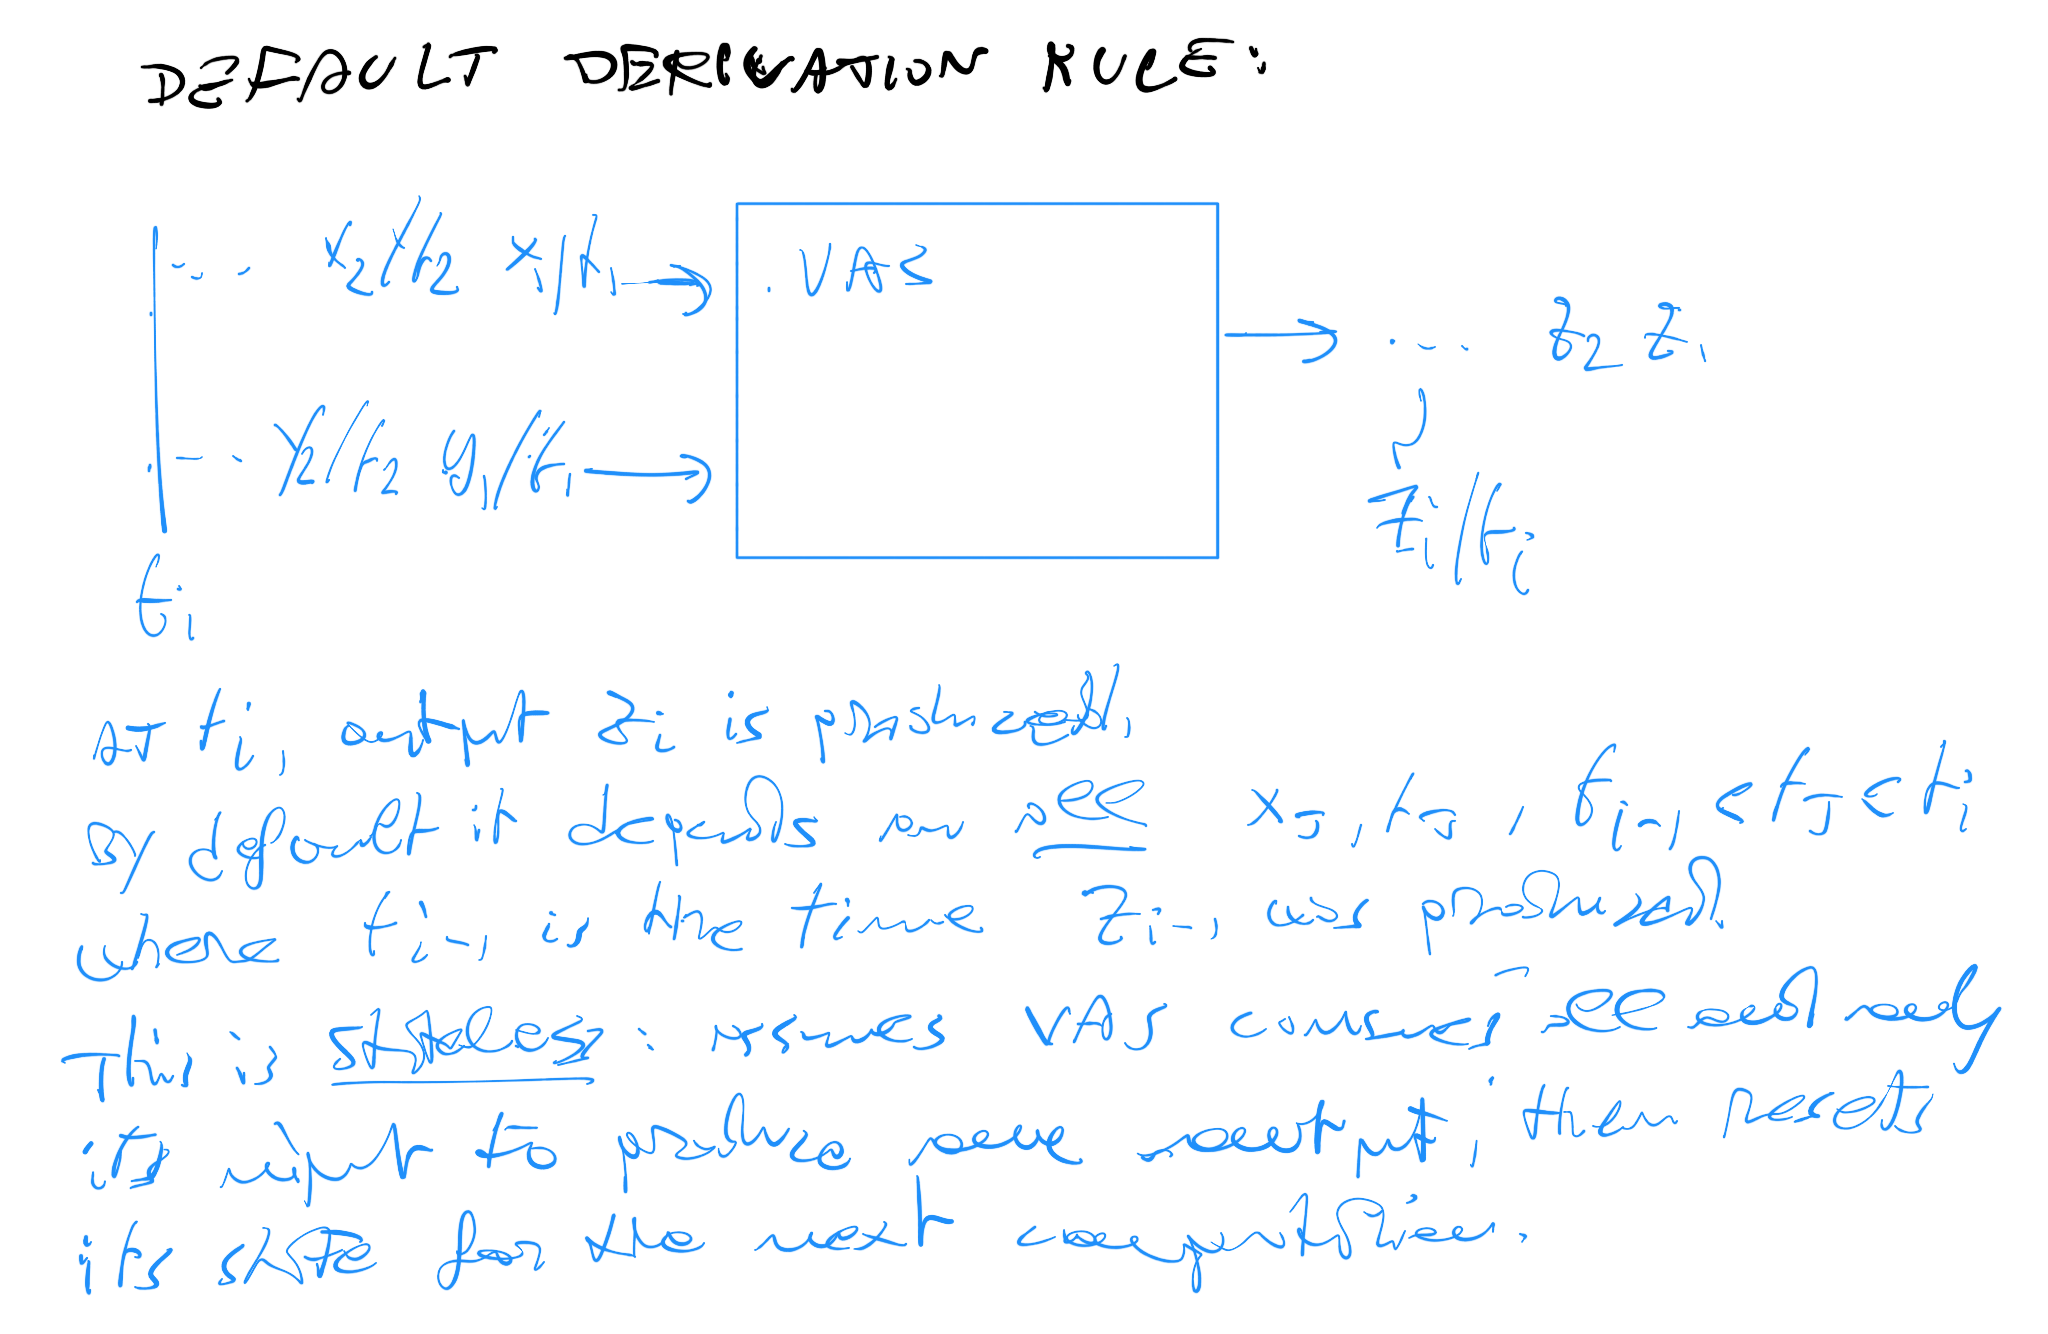
\includegraphics[width=0.7\linewidth]{./figures/black-box-aggregation-stateless}
\caption{PROV-S general pattern for stateless black box aggregations}
\label{fig:black-box-aggregation-stateless}
\end{figure*}

This needs extending to a more stateful case: outputs depends on older inputs, and outputs may depend on different windows for different inputs: see Fig. \ref{fig:black-box-aggregation-stateful}

%\begin{figure*}
%\centering
%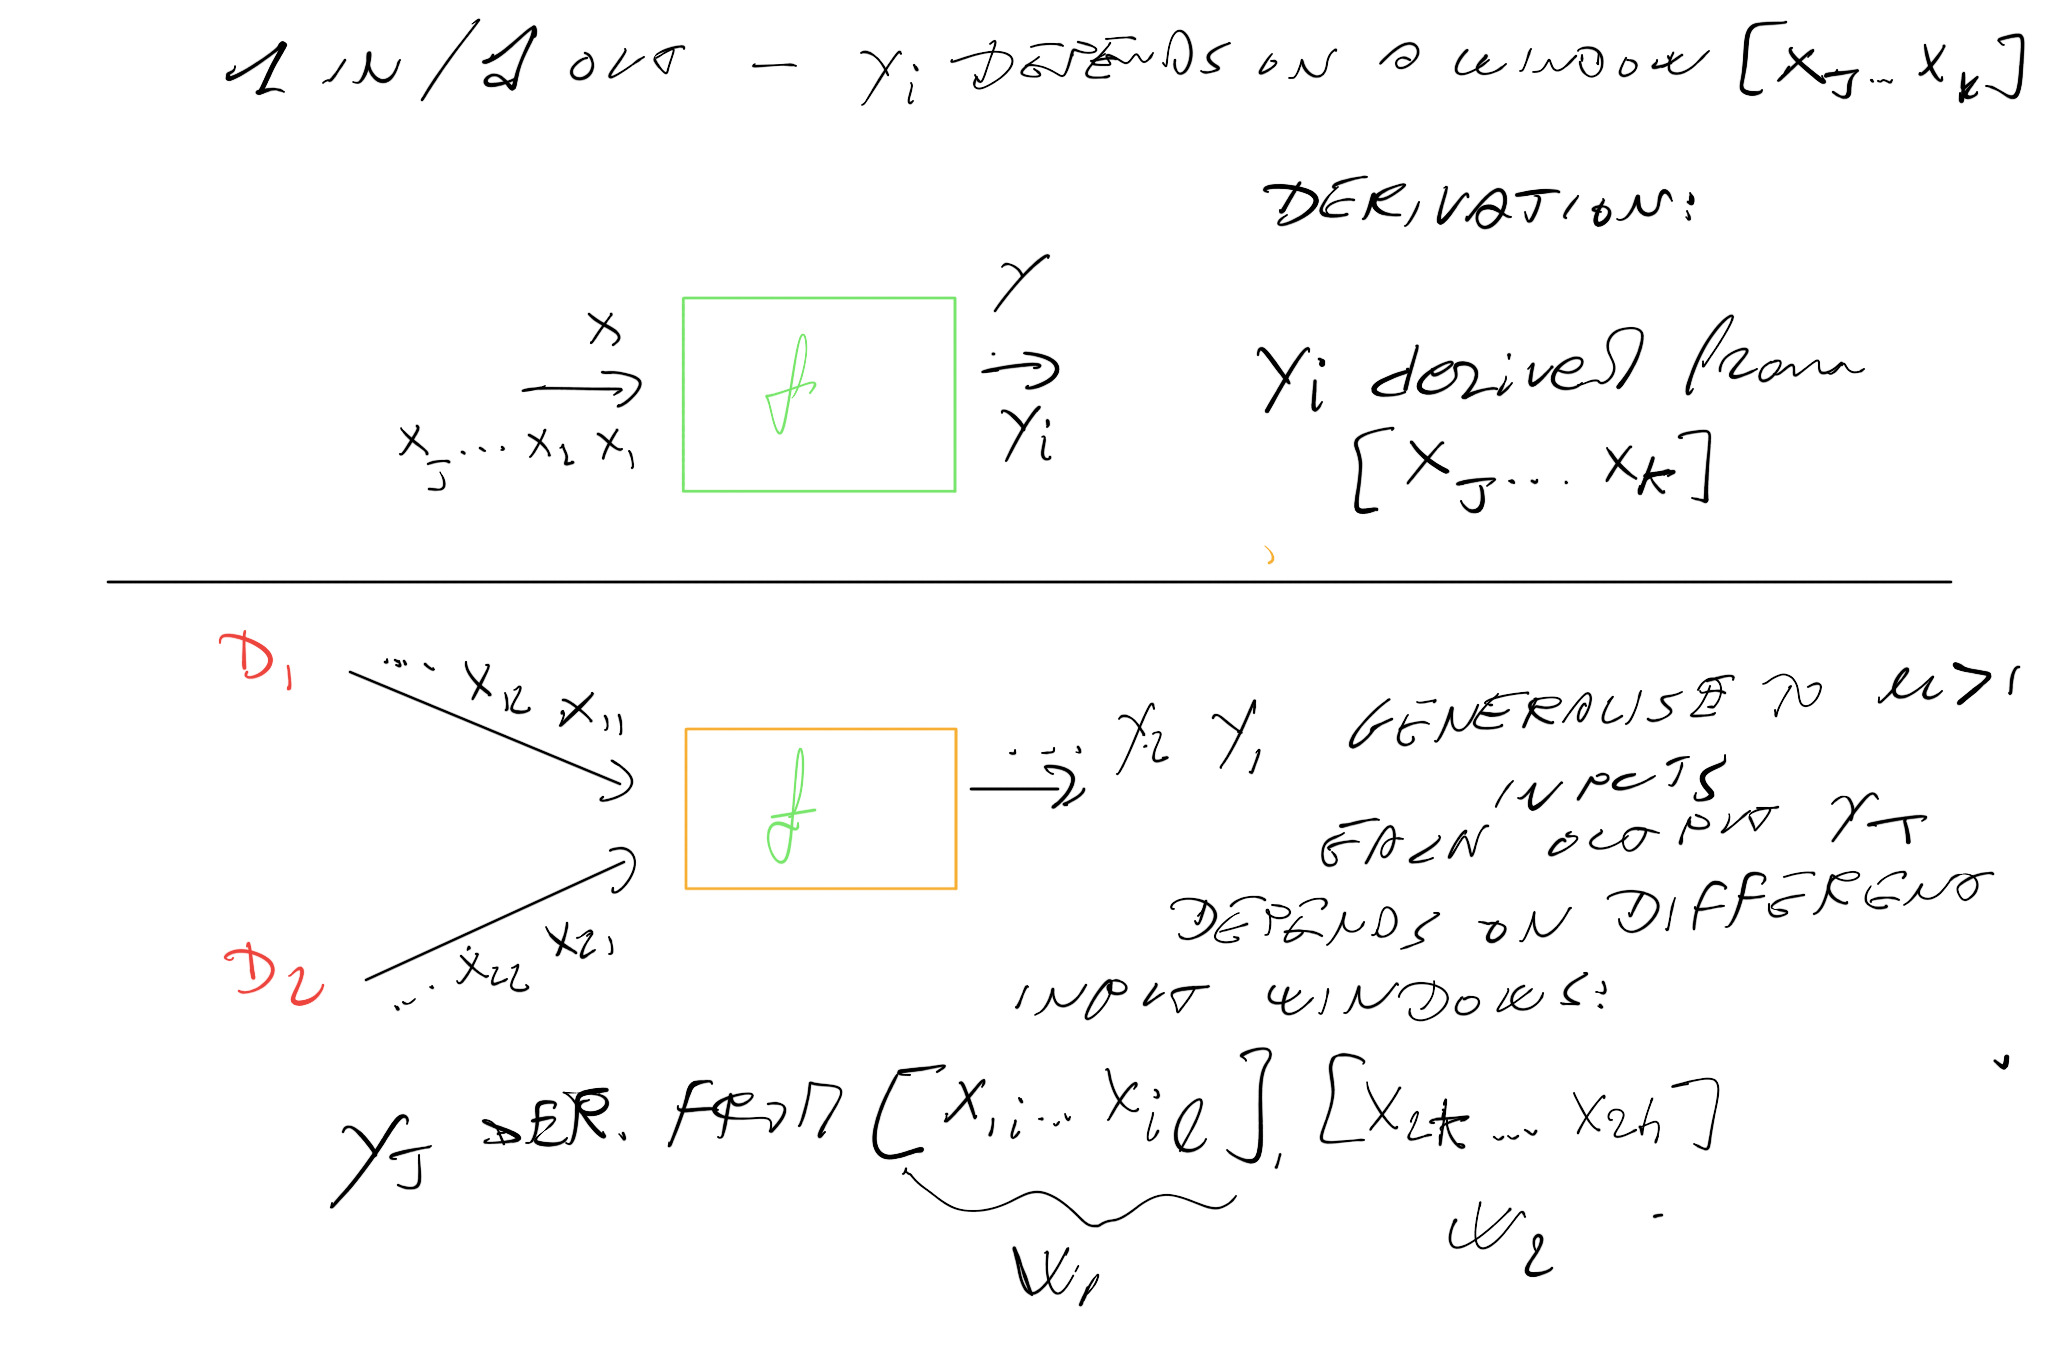
\includegraphics[width=0.7\linewidth]{./figures/black-box-aggregation-stateful}
%\caption{PROV-S general pattern for stateful black box aggregations}
%\label{fig:black-box-aggregation-stateful}
%\end{figure*}




\section{Appendix Title}

This is the text of the appendix, if you need one.

\acks

Acknowledgments, if needed.

% The 'abbrvnat' bibliography style is recommended.

\bibliographystyle{abbrvnat}

% The bibliography should be embedded for final submission.
%\bibliography{TBD}

%\begin{thebibliography}{}
%\softraggedright
%
%\bibitem[Smith et~al.(2009)Smith, Jones]{smith02}
%P. Q. Smith, and X. Y. Jones. ...reference text...
%
%\end{thebibliography}



\end{document}